\section{Credit Distribution and Distribution Strategies}
\label{section:distribution_strategies}
We now give formal definitions of data credit and Data Credit Distribution (DCD), and present three different Distribution Strategies (DSs) based on the forms of provenance discussed earlier:  Lineage-based DS, Why-Provenance-based DS, How-Provenance-based DS, \rtwo{ responsibility-based DS, and the Shapley value-based DS}.  We also show how these strategies distribute credit in the IUPHAR example discussed earlier.


\subsection{Data Credit and Data Credit Distribution}
Given a database instance $I$, a \emph{recipient of credit} is a unit of information within $I$. In the case of relational databases, recipients may be (i) the whole database; (ii) a table; (iii) a tuple; or (iv) an attribute.

\emph{Data credit} is a value $k \in \mathbb{R}_{>0}$. 
Every recipient in a database is annotated with a quantity of credit as a proxy for its importance. In this paper, we focus on {\em tuples} as recipients of credit. 

\eat{\emph{Data Credit Distribution} (DCD) considers a database instance $I$, a certain quantity of credit $k$ (here, without loss of generality, deemed to be given), 
and a query $Q$ producing a result set $Q(I)$.  
DCD consists of defining a function, i.e., a \emph{distribution strategy} (DS), to split credit into portions to be assigned to the tuples in $I$.}

Given a \emph{distribution strategy} (DS),  \emph{Data Credit Distribution} (DCD) takes a database instance $I$, a quantity of credit $k$, %(here, without loss of generality, deemed to be given), 
and query $Q$ over $I$, and it splits $k$ among the recipients of credit in $I$.

\eat{
In the following, we use the notation in \citet{CheneyProvSurvey}: a \emph{tuple location} is defined as a tuple in a relation in $I$, tagged with its name. It is indicated with $(R, t)$, where $R$ is the relation in the database, and $t$ is the tuple in $R$. With reference to the running example, \texttt{(family, $\langle f_1$, Dopamine Receptors, gpcr$\rangle$)} is the tuple location of the first tuple in the \texttt{family} relation.  The set of all the tuple locations in $I$ is called \emph{TupleLoc}.
The following is the definition of DCD at \emph{tuple level}. We refer to the level of tuple because the credit is annotated to tuples.}

In the following, we use the notation in \citet{CheneyProvSurvey}: Given a database instance $I$, a \emph{tuple location} $(R, t)$ is a tuple $t$ in  relation $R$. With reference to the running example, \texttt{(family, $\langle f_1$, Dopamine Receptors, gpcr$\rangle$)} is the tuple location of the first tuple in the \texttt{family} relation.  The set of all tuple locations in $I$ is called \emph{TupleLoc}.  We use this to formally define DCD at the \emph{tuple level}.


\begin{definition}
    \textbf{Tuple Level Data Credit Distribution (DCD)}~\citep{dosso2020data}
    \label{def:CDT}\\
    Given a query $Q$ over $I$ and $k \in \mathbb{R}_{>0}$, {DCD} is defined by the 
    function $f_{I, Q} : TupleLoc \times \mathbb{R}_{> 0} \rightarrow \mathbb{R}_{\geq0}$ such that $f_{I,Q}(t, k)=h$ where $0 \leq h \leq k$ and $\sum_{t \in TupleLoc}f_{I, Q}(t, k) = k$.  The function $f_{I Q}$ is the distribution strategy (DS).
\end{definition}

As we can see, the DS is a function that annotates each tuple in the database with a real value, which is a fraction of the given quantity $k$. The only constraint is that the sum of the credit annotations on tuples must be $k$, i.e. that no credit is generated or destroyed during the distribution.
Given $I$ and $Q$, many different DSs may be defined as long as they sum up to $k$. 

In what follows, we use information provided by data provenance to define distribution functions.
% that take into account the query over the given instance. 
For simplicity, we assume that the credit $k$ is distributed equally across the set of output tuples (i.e. the result of a query), and discuss how the credit of one output tuple $o$, $k_o$, is distributed across the instance $I$.
%We also assume that each output tuple carries a credit of 1 ($k_o=1$). 

\subsection{A Lineage-based Distribution Strategy}
%The distribution strategy is defined as follows:
In the lineage-based distribution strategy, each tuple in the output of a query distributes credit equally to each input tuple that appears in its lineage.  More formally:

\begin{definition}{Lineage-based Distribution Strategy}~\citep{dosso2020data}
    \label{def:lineage_ds}\\
    Let $I$ be a database instance, $Q$ a query over $I$, $o \in Q(I)$ an output tuple and $k_o$ the credit associated to $o$.
    Let $L$ be the lineage of $o$ and $t$ be a tuple in $I$, then $t$ receives credit equal to:
    \begin{equation*}
        f_{I, Q}(t, k_o) =  \begin{cases}
         0 & \mbox{if $t \notin L$} \\
            \frac{k_o}{|L|} & \mbox{if $t \in L$}
        \end{cases}
    \end{equation*}
\end{definition}

%It is trivial to see how this is actually a Distribution Strategy since the sum of all the values assigned by the set of functions returns exactly the value $k$:
%
%\[
%\begin{array}{ll}
%    \sum_{t \in I}f(t, k) & = \sum_{t \notin L}f(t, k) + \sum_{t \in L}f(t, k)\\
%    & = 0 + \sum_{t \in L}\frac{k}{|L|}  \\
%     & = \frac{k}{|L|}\sum_{t \in L}1 \\
%     & = k
%\end{array}{}
%\]

\eat{Definition~\ref{def:lineage_ds} 
%The DS is defined 
defines how to distribute credit $k_o$ for one tuple of the output. Therefore, to perform credit distribution for the set of output tuples (i.e. the result of a query), it is first necessary to divide the quantity of credit $k$ associated with the query among tuples in the output, and then compute the credit distribution for each tuple.
For simplicity, in this paper we assume that each output tuple carries a credit of 1 ($k_o=1$). }
Note that lineage-based DS distributes credit only to input tuples that have a role in creating $o$ by the query $Q$, and that each receives an equal share of credit. Thus, the more tuples in a lineage set, the less credit each tuple receives. 


As an example, consider the output tuples of Table \ref{table:result}, and assume that each output tuple has credit $k_o = 1$.
The lineage of the first tuple, $o_1$, is the set $\{f_1, c2f_1, c_1, c2f_2, c_2\}$. Therefore, each tuple in this set receives credit $1/5$. The other tuples of the database receive zero credit.
The lineage of the second output tuple is $\{ f_4, c2f_4, c_1\}$, therefore each of these tuples receives credit $1/3$.

At the end of the process, tuples $f_1$, $c2f_2$ and $c_2$ each receive credit $1/5$, tuples $f_4$ and $c2f_4$ receive $1/3$, while tuple $c_1$ receives $8/15$.  
Note that if a tuple appears in more than one lineage set, then it will accumulate credit from the distribution associated with each one of these sets, implying that it has a more significant role in the context $Q$, as is the case with $c_1$ in this example.
 
Not all of the tuples in the lineage of an output tuple are necessary to be present at the same time for the output tuple to appear in the query results.  For example, if the database only had the set of  tuples $\{f_1, c2f_1, c_1\}$ or the set $\{f_1, c2f_2, c_2\}$, the existence of $o_1$ would still be guaranteed. 
In other words, while $f_1$ is always needed for $o_1$ to appear in the output, 
only one of the sets of tuples $\{ c2f_1, c_1 \}$ and $\{ c2f_2, c_2 \}$ is required. 
One could therefore argue that it would be more fair for $f_1$ to receive more credit than the other four tuples, given its role in producing $o_1$.  

This highlights one limitation of the lineage-based DS: while able to find all and only the relevant tuples of the output, it does not distinguish the \emph{importance} of tuples in the query computations. 
%This information could be incorporated in the definition of a DS to distribute credit based on the actual role that tuples play in the computation. 
We therefore present four other, more sophisticated, forms of distribution strategies based on why-provenance, how-provenance, \rtwo{ responsibility, and Shapley value}.

\subsection{A Why-Provenance-Based Distribution Strategy}
The distribution strategy based on why-provenance first equally distributes the credit $k_o$ among the witnesses of the witness basis for $o$, and then equally divides the credit of a witness among the tuples in the witness. 
Since a tuple may appear in more than one witness, it will receive more than one portion of credit from the same distribution. More formally:

%The distribution strategy based on why-provenance is defined as follows:

 \begin{definition}{Why-Provenance-based Distribution Strategy}\\
        \label{def:why_distribution}
    Let $I$ be a database instance, $Q$ a query over $I$, $o \in Q(I)$ an output tuple and $k_o$ the total credit associated to $o$. 
    Let $\mathcal{W} = Why(Q, I, o)$ be the witness basis of $o$ according to $Q$ and $I$, and $W \in \mathcal{W}$ be a witness. 
    
    \eat{
    Let $\gamma(\mathcal{W}, t): (\mathcal{W}, t) \mapsto \mathcal{P}(\mathcal{P}(TupleLoc))$ be the function that returns the set 
    $\{W \in \mathcal{W} : t \in W\}$.
    % of all the witnesses $W \in \mathcal{W}$ such that $t \in W$.
    }
 
    Then tuple $t$ in $I$ receives credit equal to:
    \begin{equation*}
        f_{I, Q}(t, k_o) =
            \frac{k_o}{|\mathcal{W}|}\sum_{W \in \gamma(\mathcal{W}, t)}\frac{1}{|W|}
    \end{equation*}            
    where $\gamma$ is a function which returns all witnesses $W$ in which $t$ appears:
   $$\gamma(\mathcal{W}, t)=  \{W \in \mathcal{W} : t \in W\}$$
\end{definition}
%We now prove that this set of functions is a Distribution Strategy. As we can see, with abuse of language we use $t \notin \mathcal{W}$ to indicate the input tuples $t$ that are not present in any witness.
%\[
%\begin{array}{rl}
%\sum_{t \in I}f_{I, Q}(t, k) & = \sum_{t \notin \mathcal{W}}f_{I, Q}(t, k) + \sum_{t \in \mathcal{W}} f_(I, Q)(t, k)\\
%                    & = 0 + \frac{k}{|\mathcal{W}|}\left[\sum_{W \in  \mathcal{W}} \left(\sum_{t \in W}\frac{1}{|W|}\right)\right]\\
%                    & \frac{k}{|\mathcal{W}|}\sum_{W \in  \mathcal{W}} 1 \\
%                    & = \frac{k}{|\mathcal{W}|}|\mathcal{W}|\\
%                    & = k
%\end{array}
%\]

\begin{figure}[]
\centering
  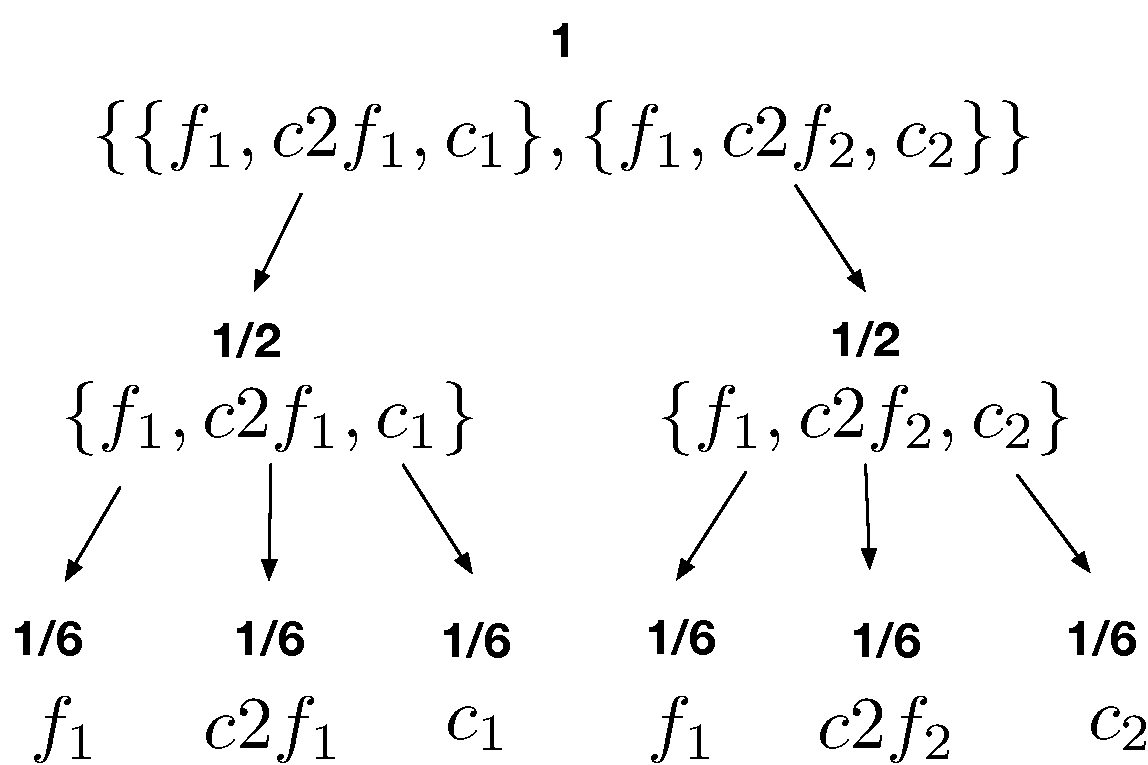
\includegraphics[width=.45\textwidth]{figures/why_distribution}
  \caption{Distribution of credit using why-provenance-based DS for tuple $o_1$.}
  \label{figure:why_prov_distribution}
\end{figure}

Figure \ref{figure:why_prov_distribution} shows the distribution of credit with why-provenance-based DS for tuple $o_1$.
The credit is first equally divided between the two witnesses, so that both receive credit $1/2$. 
The credit is then further divided among the tuples in each witness. Since each witness has three tuples, each tuple in a witness receives $1/6$ of credit. At the end of the distribution, $f_1$ receives a total credit of $1/3$, and the other tuples receive $1/6$ each.
This distribution better reflects the role of $f_1$ in the generation of $o_1$ since, as discussed earlier, it is the only mandatory tuple for $o_1$ to appear in the output; only one of the two other pairs of tuples are necessary for $o_1$ to appear in the result. 

This example illustrates that why-provenance can better reward input tuples depending on their role. Tuples that appear in more than one witness are rewarded more than others. 
\eat{This means that tuples that are more important to the generation of the output, since they are used more by the query, are rewarded more than tuples that are ``interchangeable'' with others. }

\subsection{A How-Provenance Based Distribution Strategy}
\label{section:how_prov_distr_tuples}

%\scream{You did not talk about coefficients in section 4, you only talked about monomials.}

%How-provenance conveys more information than why-provenance since it not only captures what tuples are relevant to the output and in which combination, but also how they are used. The ``how" is captured through the provenance polynomials.

The how-provenance-based DS first distributes the credit to the monomials of the polynomial accordingly to the weight represented by their coefficients, then to the tuples of each monomial accordingly to the weights represented by their exponents. 

To define the DS more formally, we introduce some notation and illustrate it using the provenance polynomial $\mathcal{H}$ shown in Figure \ref{figure:how_example}. This notation is also shown  in Table \ref{tab:notation} for easy reference.


\begin{figure}[]
\centering
  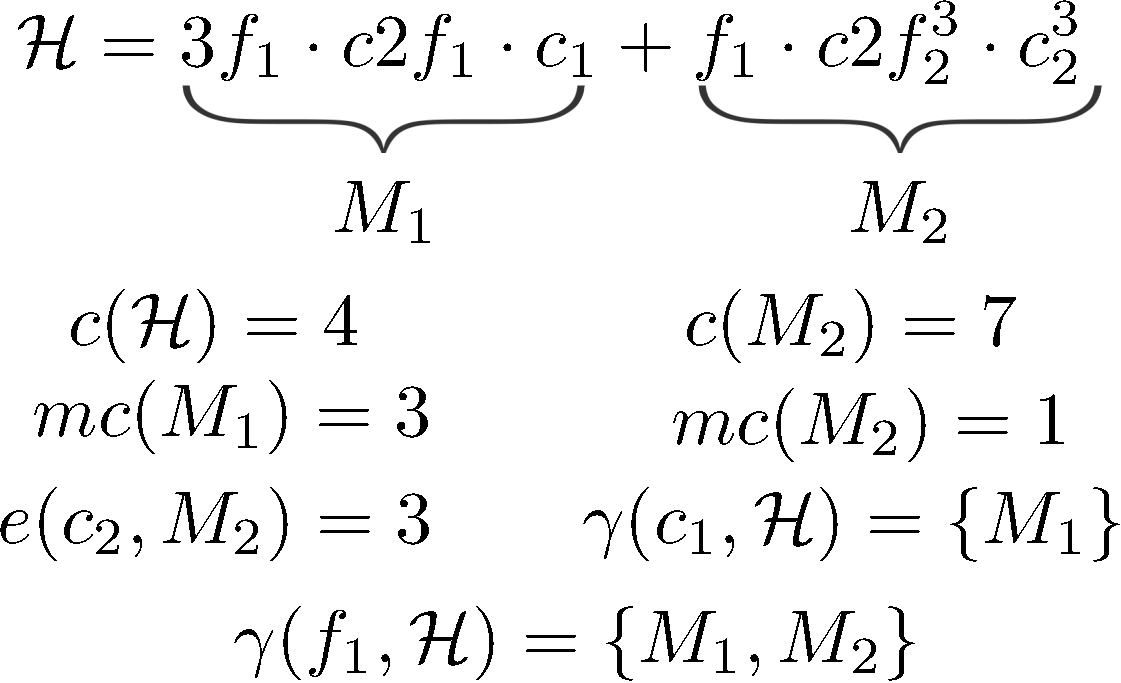
\includegraphics[width=.4\textwidth]{figures/how_example}
  \caption{Illustration of notation used to define the how-provenance based DS } %in Definition \ref{def:how_distribution}.}
  \label{figure:how_example}
\end{figure}

%In this figure we show the notation that we use to refer to different information taken from the provenance polynomial. 
We call $c$ the function that, given a polynomial, returns the sum of its coefficients; thus $c(\mathcal{H})=\;3+1=4$. 
\rone{We call $e$ the function that, given a monomial, returns the sum of its exponents, thus $e(M_2)=1+3+3=7$.}
$mc$ is the function that takes as input a monomial and returns its coefficient; thus $mc(M_1) = 3$. 
\rone{$te$ is a function that takes as input a tuple and a monomial, and returns the exponent of the tuple in the monomial, if present; thus $te(c_2, M_2)=3$}. 
Finally, $\gamma$ takes as input a tuple and the whole polynomial, and returns a set of monomials containing that tuple, if present in the polynomial; thus $\gamma(f_1, \mathcal{H})=\;\{M_1, M_2\}$, $\gamma(c_2, \mathcal{H})=\;\{M_2\}$. 

\eat{
%\scream{This needs to be simplified.  Get rid of the mathematical notation and just give an English definition.}
More formally, consider the provenance polynomial $\mathcal{H} = H(Q, I, o)$ of a tuple $o$. We define: 
\begin{enumerate}
	\item $c(\mathcal{H}) = n$ the function $c: \mathbb{N}[TupleLoc] \mapsto \mathbb{N}$ that, given a polynomial, returns the sum of its coefficients;
	\item $c(M)$ the function $c: \mathcal{M} \mapsto \mathbb{N}$ that, given a monomial $M$, returns the sum of its exponents (with $\mathcal{M} \subset \mathbb{N}[TupleLoc]$ such that $\mathcal{M}$  is made only by the monomials $M$ in $\mathbb{N}[TupleLoc]$); 
	\item $e(t, M)$ the function $e: TupleLoc \times \mathcal{M} \mapsto \mathbb{N}$ that, given in input a tagged tuple and a monomial, returns the exponent of that tuple inside the monomial;
	\item $mc(M)$ the function $mc: \mathcal{M} \mapsto \mathbb{N}$ that, given in input one monomial, returns its coefficient;
	\item $\gamma(t, \mathcal{H})$ the function $\gamma: TupleLoc \times \mathbb{N}[TupleLoc] \mapsto \mathcal{M}$ that, given a tuple $t$ and a provenance polyomial $\mathcal{H}$, returns the (possibly empty) set of monomials $M$ in $\mathcal{H}$ such that $t$ appears in $M$.
\end{enumerate}
}
%\scream{You need to give a little example to clarify the ideas.}
\begin{definition}{How-Provenance-Based Distribution Strategy}
    \label{def:how_distribution}\\
    Let $I$ be a database instance, $Q$ a query over $I$, $o \in Q(I)$ an output tuple, $\mathcal{H}$ be the provenance polynomial for $o$, and $k_o$ the credit given to $o$.
    The credit given to tuple $t$ in $I$ is:
    \[
    f_{I, Q}(t, k_o) = \frac{k_o}{c(\mathcal{H})} \sum_{M \in \gamma(t, \mathcal{H})} mc(M) \frac{\rone{te(t, M)}}{\rone{e(M)}}
    \]
\end{definition}

%We demonstrate that this is a Distribution Strategy by considering the contributions of the single monomials one at a time in the sum. With abuse of language in the following demonstration, we write $t \in M$ to indicate one tuple $t$ appearing in the monomial $M$.
%
%\[
%\begin{array}{rl}
%\sum_{t \in I}f(t, k) & = \sum_{t | \gamma(t, \mathcal{H}) = \emptyset}f(t, k) + \sum_{t | \gamma(t, \mathcal{H}) \neq \emptyset}f(t, k) \\
%    & = 0 + \sum_{M \in l(\mathcal{H})} \left(k \cdot \frac{mc(M)}{c(\mathcal{H})} \sum_{t \in M} \left[\frac{e(t, M)}{c(M)} \right]\right)\\
%    & = \frac{k}{c(\mathcal{H})}\sum_{M \in l(\mathcal{H})} \left[ \frac{mc(M)}{c(M)} \sum_{t \in M} e(t, M)  \right] \\
%    & = \frac{k}{c(\mathcal{H})} \sum_{M \in l(\mathcal{H})} mc(M)\\
%    & = k
%\end{array}
%\]

\eat{The how-provenance-based DS first distributes the credit to the monomials of the polynomial accordingly to the weight represented by their coefficients, then to the single tuples in every monomial accordingly to the weights represented by their exponents. }

Going back to the example of Table \ref{table:result_how_prov}, consider $o_1$ with provenance polynomial $f_1 c2f_1 c_1 + f_1 c2f_2 c_2$. The how-provenance-based DS firstly divides the credit between the two monomials. Since the coefficients of each monomial are $1$, the credit is split in half. If they were, for example, $1$ and $2$ respectively, $1/3$ of the credit would go to the first monomial, and $2/3$ to the second.  
Since in our example each variable has exponent $1$, the credit is further divided equally among the three variables. Thus, at the end of the computation, $f_1$ receives $1/3$, and the other tuples receive $1/6$.

% \rone{Consider instead the example where the polynomial is $f_1^2 c2f_1 c_1 + f_1^2 c2f_2 c_2$, $k_0 = 1$, and let us focus on the first monomial. It receives $1/2$ of credit, then $f_1$ receives $1/4$ of credit due to its exponent, while the other two tuples receive $1/8$.}
%If, for example, the first monomial was $f_1^2 c2f_1 c_1$, then the portion of credit of this monomial would be divided in this way: $1/2$ to $f_1$ and $1/4$ to each of the other two tuples. 


In this specific example, the how-provenance-based DS has the same outcome as the one based on why-provenance. %Consequently, one may ask if there is a significant difference between the two strategies. 
We therefore consider another query over GtoPdb, \texttt{Q2}, that asks for the families of type \texttt{gpcr} that have as contributor a researcher located in the UK:

\vspace{2mm}
{\footnotesize
\begin{adjustwidth}{25pt}{5pt}
\begin{verbatim}
	Q2: SELECT DISTINCT F.name 
	FROM family as F JOIN
		(SELECT DISTINCT f.name AS name
		FROM family AS f JOIN contributor2family AS c2f ON f.id = c2f.family_id
		JOIN contributor AS c ON c2f.contributor_id = c.id
		WHERE c.country = "UK") AS R ON F.name = R.name
	WHERE F.type = "gpcr"
\end{verbatim}	
\end{adjustwidth}
}
\vspace{2mm}

\begin{table}[]
\centering
  \begin{tabular}{|l||c|}
  \hline
    id & name\\
    \hline
    $oxs_1$ &  Dopamine Receptors\\
    \hline
  \end{tabular}
  \newline
\vspace{2mm}
  \begin{tabular}{c | c | c}
  	lineage & why-provenance & how-provenance   \\
  	$\{f_1, c2f_1, c_1, c2f_2, c_2\}$ & $\{\{f_1, c2f_1, c_1\}, \{f_1, c2f_2, c_2\}\}$ & $f_1^2 c2f_1 c_1 + f_1^2 c2f_2 c_2$\\
  \end{tabular}
    \caption{Result of query \texttt{Q2} applied on the database of Table \ref{table:running_example} and its different provenances. The reported numbers are the credit distributed through the process.}
  \label{table:difference_result}
\end{table}

The result of \texttt{Q2} is shown in Table \ref{table:difference_result}, and consists of one tuple, $oxs_1$, annotated with each of the three provenances. As can be seen, lineage and why-provenance are identical to those of the tuple $o_1$ in the previous example. 
The how-provenance, however, is different since tuple $f_1$ is used twice: first in the join of the inner query, and second in the join of the outer query. This information is lost in the first two forms of provenances since they are sets, but it is captured in how-provenance through the use of the operator `$\cdot$'.

%\scream{This polynomial still doesn't have coefficients other than 1, but ok. Why don't you rewrite the polynomial to $f_1^2c2f_1c_1 + f_1^2c2f_2c_2$ to make the exponents clearer?}

\begin{figure}[]
  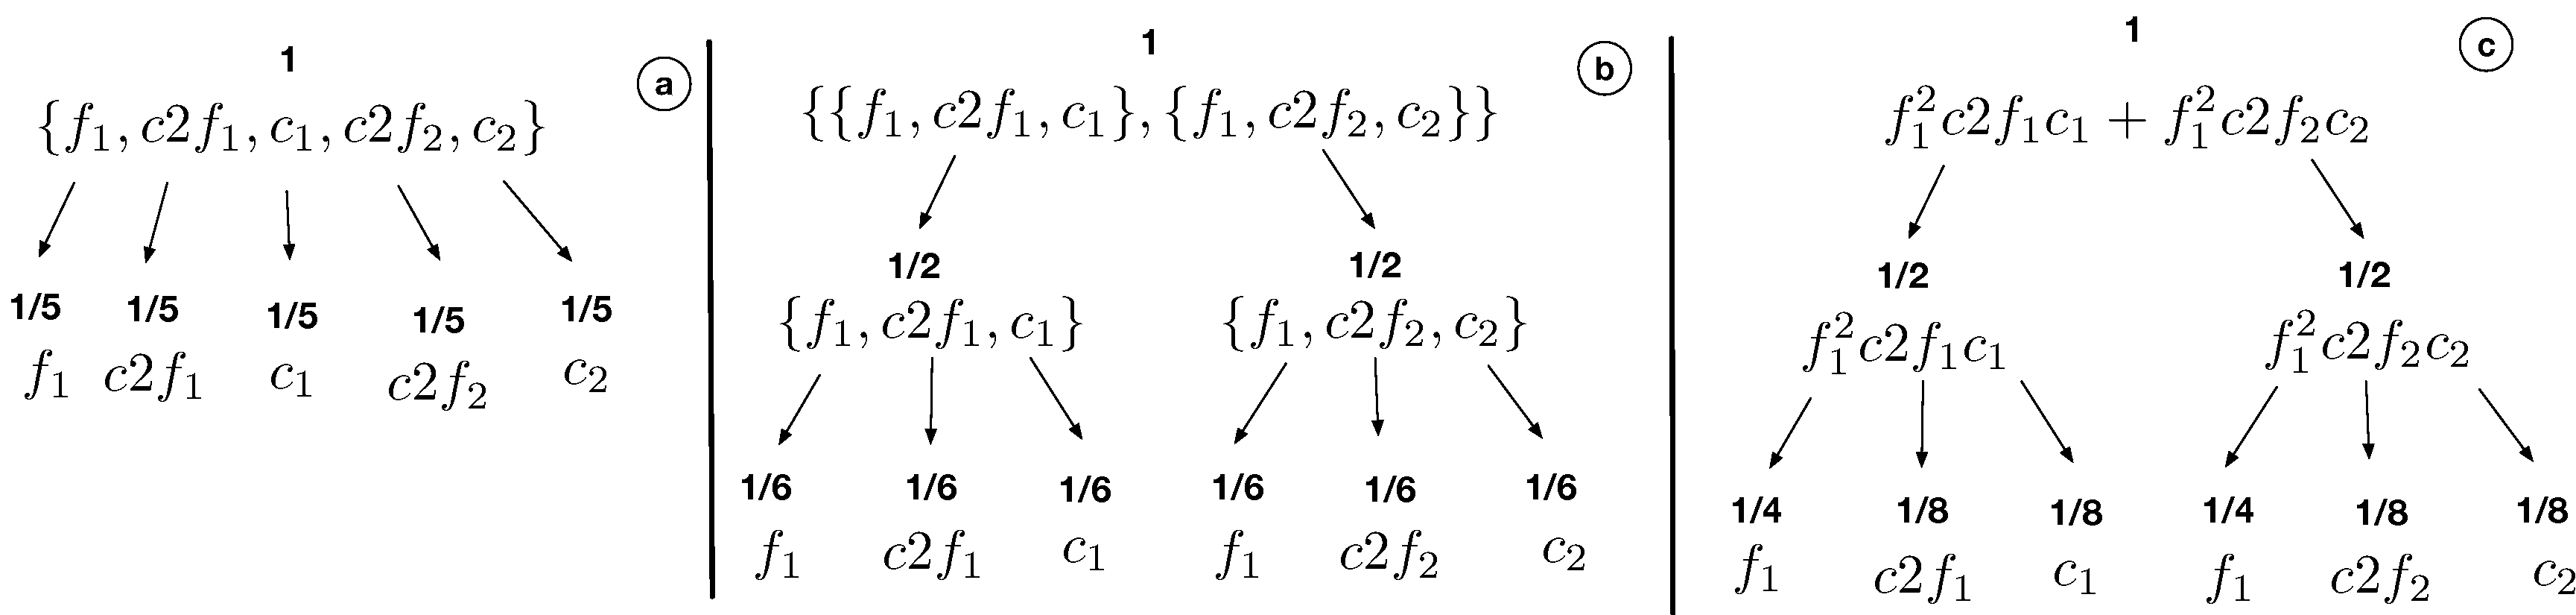
\includegraphics[width=\textwidth]{figures/how_distribution}
  \caption{Comparison of different distributions strategies for tuple $o_1$ produced by query \texttt{Q2}.}
  \label{figure:distributions_differences}
\end{figure}


Figure \ref{figure:distributions_differences} shows the differences between the three DS for the tuple $o_1$ of Table \ref{table:difference_result}. Subfigure \ref{table:difference_result}.a uses lineage, sub-figure \ref{table:difference_result}.b uses why-provenance, and sub-figure \ref{table:difference_result}.c uses how-provenance. 
The DS based on the provenance polynomial gives credit $1/2$ to $f_1$, and $1/8$ to the other tuples.
This is reasonable since \texttt{Q2} relies on $f_1$ even more than \texttt{Q1} does. 
The distribution based on how-provenance rewards $f_1$ more, showing that how-provenance is even more sensitive to the tuples' role in a query than why-provenance. %In this case, the why-provenance is not sensible to this difference. 
This is a direct consequence of the fact that, as proven in \citep{howProvenanceGreen}, how-provenance is more general than why-provenance and lineage, in the sense that it contains more information. 

\rtwo{\subsection{Responsibility-based Distribution Strategy}}
% Given the lineage of an output tuple $o$, it is first possible to compute the type of causality of each of tuple in its lineage, distinguishing between counterfactual and actual causes, by testing what happens as a result of removing single tuples and contingency sets of other tuples of the lineage.
% It is then possible to compute their responsibility through the minimal contingency sets found in this way. 

% One possible option for defining a distribution strategy using responsibility is to simply assign the responsibility of a tuple as its credit. In this way, responsibility is both a way to compute credit and to distribute it.
% Using the example of Table \ref{table:result_responsibility}, in the case of output tuple $o_1$, $f_1$ receives credit 1 and the other tuples receive credit $0.5$. 

As described in Section \ref{sec:responsibility}, causality and responsibility is 
new information that is added to lineage.   One possible option for defining a distribution strategy using responsibility is to simply assign the responsibility of each tuple in the lineage of an output tuple as its credit. In this way, responsibility is both a way to compute credit and to distribute it.
Using the example of Table \ref{table:result_responsibility}, in the case of output tuple $o_1$, $f_1$ receives credit 1 and the other tuples receive credit 0.5.


However, we want a DS that is also a function of the input credit value $k$ in order to be comparable with the other three strategies proposed so far.
We define a new DS based on responsibility that is a function of the quantity of credit $k_o$ that assigns to each tuple of the lineage a portion of this credit weighted by its normalized quantity of responsibility.
This will give a bigger portion of credit to tuples that are higher in the responsibility ranking.
Formally:
\newline
\begin{definition}{Responsibility-based Distribution Strategy}\\
\label{def:resp_ds}
Let $I$ be a database instance, $Q$ a query over $I$, $o \in Q(I)$ an output tuple, $L$ the lineage of $o$, and $k_o$ the credit given to $o$. The credit given to tuple $t$ in $I$ is:
\[
	f_{I, Q}(t, k_o) = k_o \frac{\rho_t}{\sum_{t' \in L} \rho_{t'}}
\]
where $\rho_j$ is the responsibility of tuple $j$ as in Definition \ref{def:responsibility}.
\end{definition}


\begin{figure}[]
\centering
  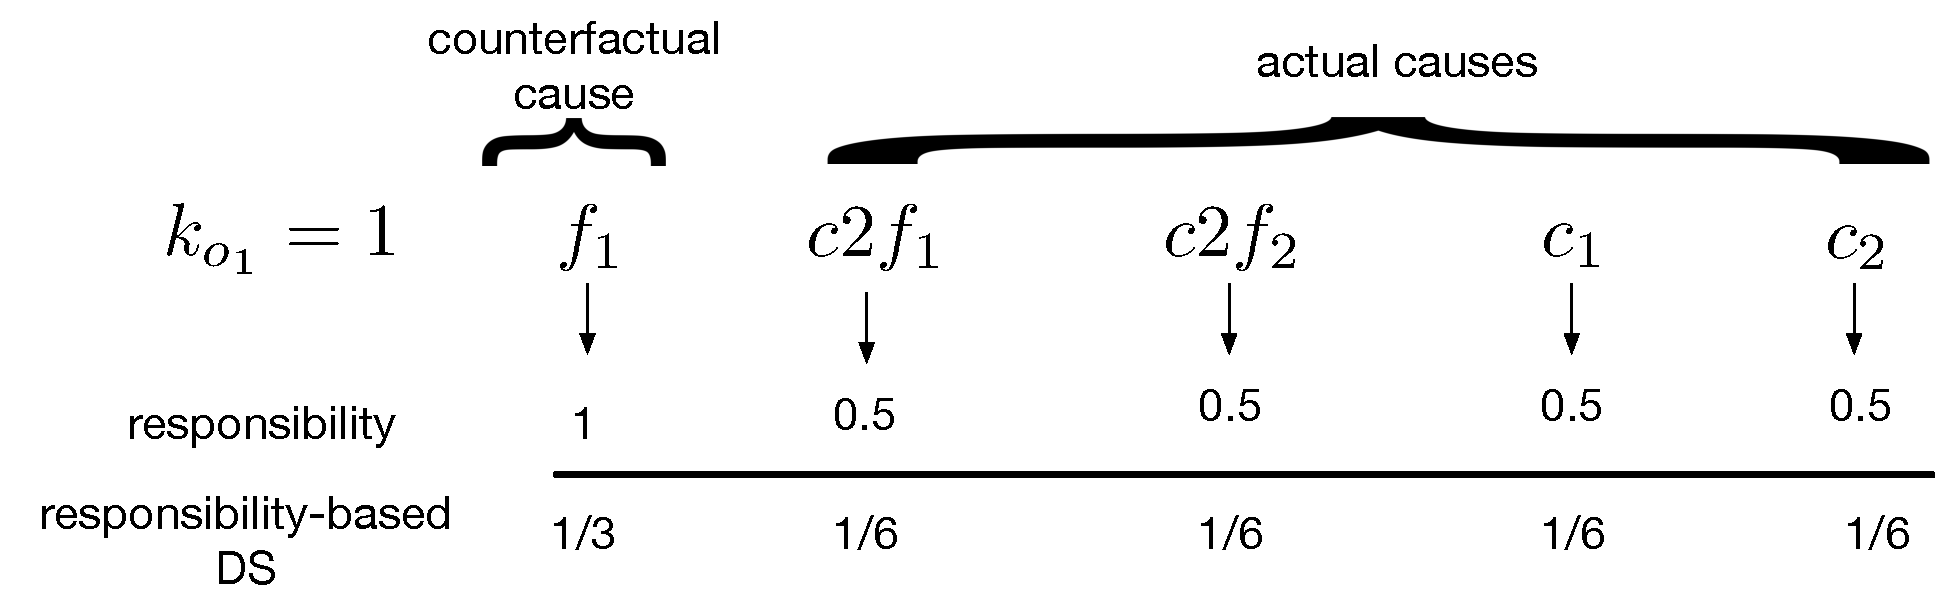
\includegraphics[width=.7\textwidth]{figures/resp_example}
  \caption{Example of distribution of credit using 
%  responsibility and normalized responsibility and 
    the responsibility-based DS, assuming $k_o = 1$.}
  \label{fig:resp_example}
\end{figure}

Note that only the tuples that belong to the lineage will receive a quantity of credit $> 0$. Furthermore, the more important the tuple is, i.e., the higher its responsibility, the larger the quantity of credit received. 

Figure \ref{fig:resp_example} shows the responsibility and credit assigned to the tuples of the lineage of the output tuple $o_1$ of Table \ref{table:result_responsibility}. 
Assuming that $k_{o_1} = 1$, $f_1$ receives credit $1/3$, while the others receive credit $1/6$. 
As we see, the DS in this case returns the same distribution as that obtained using why-provenance as shown in Figure \ref{figure:distributions_differences}.
This is not always the case though, as we show in the example of Section \ref{sec:synth_queries}.

\rtwo{\subsection{Shapley value-based Distribution Strategy}}

As with responsibility, the Shapley value can be seen both as a method to generate and distribute credit. Moreover, it can be seen that, using the definition of Shapley value for Boolean queries given in Section \ref{sec:shapley_value}, the sum of the Shapley values of all the tuples of the lineage $L$ of an output tuple $o$ is $1$. Thus, the definition of a Shapley value-based distribution strategy is straightforward:

\begin{definition}{Shapley Value-Based Distribution Strategy} \\
	Let $I$ be a database instance, $Q$ a query over $I$, $o \in Q(I)$ an output tuple, and $k_o$ the credit given to $o$. The credit given to tuple $t$ in $I$ is:
	\[
		f_{I, Q}(t, k_o) = k_o \cdot 
		Shapley(\bar{Q}_o, I, t)
	\] 
	where $\bar{Q}_o$ is the Boolean query such that, given the set of facts $D$, $\bar{Q}_o(D) = 1$ if and only if $o$ is in the output of $Q$ on $D$.
\end{definition}

As shown in Table \ref{table:result_shapley}, tuple $f_1$ in $o_1$'s lineage takes credit $7/15$ when $k_{o_1} = 1$, while the other tuples of the lineage take credit $2/15$. This DS still rewards $f_1$ more than the other tuples, since it is more important than the other tuples of the lineage. This DS thus behaves differently from all the other four previous strategies. In particular, $f_1$ is rewarded more with this DS than with the others.

In the case of $o_2$ there is only one witness set, thus this DS behaves like all the others, distributing $1/3$ of credit to each tuple in the lineage. 








